\section{Convolution and Pooling (10 Points)}

\begin{figure}[H]
    \centering
    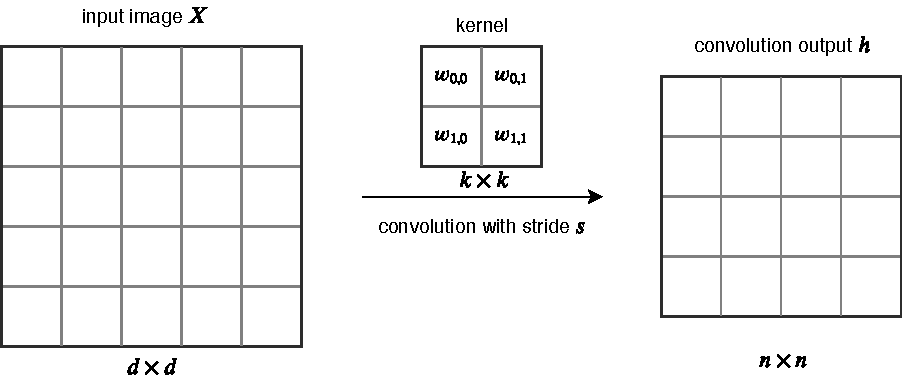
\includegraphics[width=0.7\textwidth]{images/conv.pdf}
    \caption{A simple example of convolution.}
    \label{fig:conv}
\end{figure}

In this problem, you will work on derivations of convolution. You will also get familiar with \texttt{im2col} (image to column), a popular technique to accelerate convolution. For this problem, assume padding = 0.

% \texttt{Im2col} is a method of representing convolution as matrix multiplication. Since we can do this, we know that convolution is a \textbf{linear operation}.\\

\subsection{(3 pts)} 
In lecture, you learned about two types of pooling as forms of downsampling: Max Pooling and Average Pooling
\begin{enumerate}
    \item
    Please show that \textbf{Average Pooling} is a linear operator by describing how it can be represented as a Convolution. In particular, for a square pooling field of shape $(p,p)$, please define the kernel matrix $A$ and stride $s$ needed to \textbf{implement Average Pooling as Convolution} for a one-channel input.
    \item
    Additionally, please explain why \textbf{Max Pooling} cannot be implemented as a convolution.
    \item
    Please say which you think would perform better and why: a CNN made up of \textbf{Convolutions and Max Pools} or a CNN made up of \textbf{Convolutions and Average Pools}.
\end{enumerate}
\newpage
    
\begin{soln}{height=10cm}
\FourA
\end{soln}
    

\subsection{(4 pts)} 

Let the input $X \in \mathbb{R}^{d\times d} $ be one single image, and is convolved by a $k\times k$ kernel with stride $s$. A simple example is shown in Figure \ref{fig:conv}.


\begin{enumerate}[label=\alph*.]
\item \textbf{(1 pts)} The convolution output is in the shape of $n\times n$. Can you represent the output dimensionality $n$ in terms of $d$, $k$ and $s$?

\begin{soln}{height=3cm}
\FourBA
\end{soln}
    
\item \textbf{(1 pts)} Denote the loss as $L$, convolution output as $h$, and kernel parameters as $w$. During backpropagation, given $\frac{\partial L}{\partial h_{i, j}}$ and input $X$, please derive $\frac{\partial L}{\partial w_{a, b}}$.

\begin{soln}{height=3cm}
\FourBB
\end{soln}

\pagebreak 
\item \textbf{(2 pts)} Can the above derivative be represented as a convolution? If so, write down its expression and define the corresponding kernel.

\begin{soln}{height=15cm}
\FourBC
\end{soln}

\end{enumerate}


\pagebreak

\subsection{(3 pts)}
In this part, you will be walked through \texttt{im2col} (image to column), and you are encouraged to use this technique in the programming exercise. Naively, an simple implementation of convolution would be sliding the kernel over the feature map. However, this would result in loops of all kernels and all locations, which is slow and can be accelerated by constructing two big matrices and going through one single matrix multiplication.

\begin{figure}[H]
    \centering
    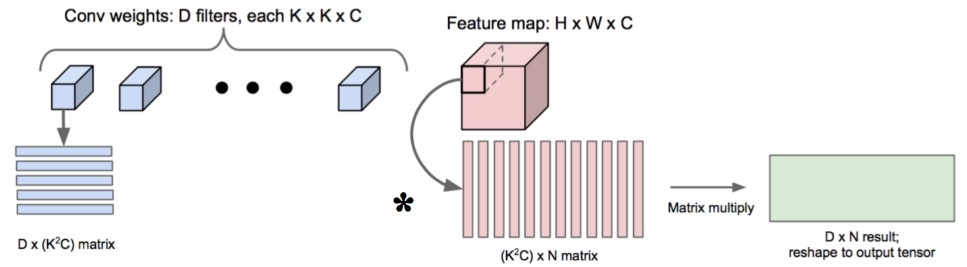
\includegraphics[width=0.9\textwidth]{images/im2col.jpg}
    \caption{Illustration of im2col.}
    \label{fig:im2col}
\end{figure}

An illustration of im2col is shown in Figure \ref{fig:im2col}. A patch inside the feature map corresponds to a possible location of the kernel. Each patch is of the same size as the convolution kernel, $K^2 C$, and $N$ is the number of all possible locations, or in other words, the spatial size of the output. We can take all possible patches, and reshape them into column vectors, then concatenate the vectors into one big matrix. Similarly, we can reshape the kernels into row vectors, and concatenate them into another one. Then we only need to go through one single matrix multiplication. And reshape the result to output shape.

For example, if the input feature map is of shape $32\times 32\times 3$, and we apply 5 filters each of size $5\times 5\times 3$ with stride=1 and padding=2, then the filter matrix would be of size $5\times 75$, and image matrix would be of size $75\times 1024$. The multiplication result would be of size $5\times1024$, and we need to reshape the result to shape $32\times 32\times 5$. (Hint: be very careful during reshaping.) 

\pagebreak

\begin{enumerate}[label=\alph*.]
\item \textbf{(2 pts)} Consider a toy example where the input feature map is of size $3\times3$, and convolved by 2 kernels of size $2\times2$ with stride $s=1$, as shown in Figure \ref{fig:toy_im2col}, please write the two constructed matrices with im2col.

\begin{figure}[H]
    \centering
    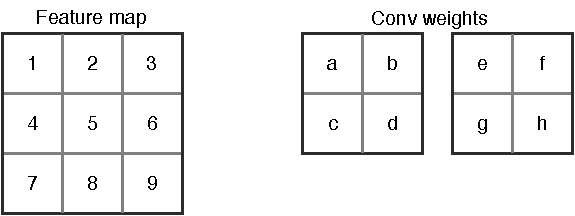
\includegraphics[width=0.5\textwidth]{images/im2col_toy_sample.pdf}
    \caption{A toy example of im2col}
    \label{fig:toy_im2col}
\end{figure}

% \item Problem about gradient.

\begin{soln}{height=5cm}
\FourCA
\end{soln}

\item \textbf{(1 pts)} Give one significant drawback of im2col.

\begin{soln}{height=5cm}
\FourCB
\end{soln}

\end{enumerate}